\documentclass[14pt]{extreport}
\usepackage{gost}
\usepackage{graphicx}
\usepackage[toc, page]{appendix}
\usepackage{multicol}


\begin{document}
\setlength{\parindent}{1.25cm} % для шрифта 14pt
\pagestyle{empty}
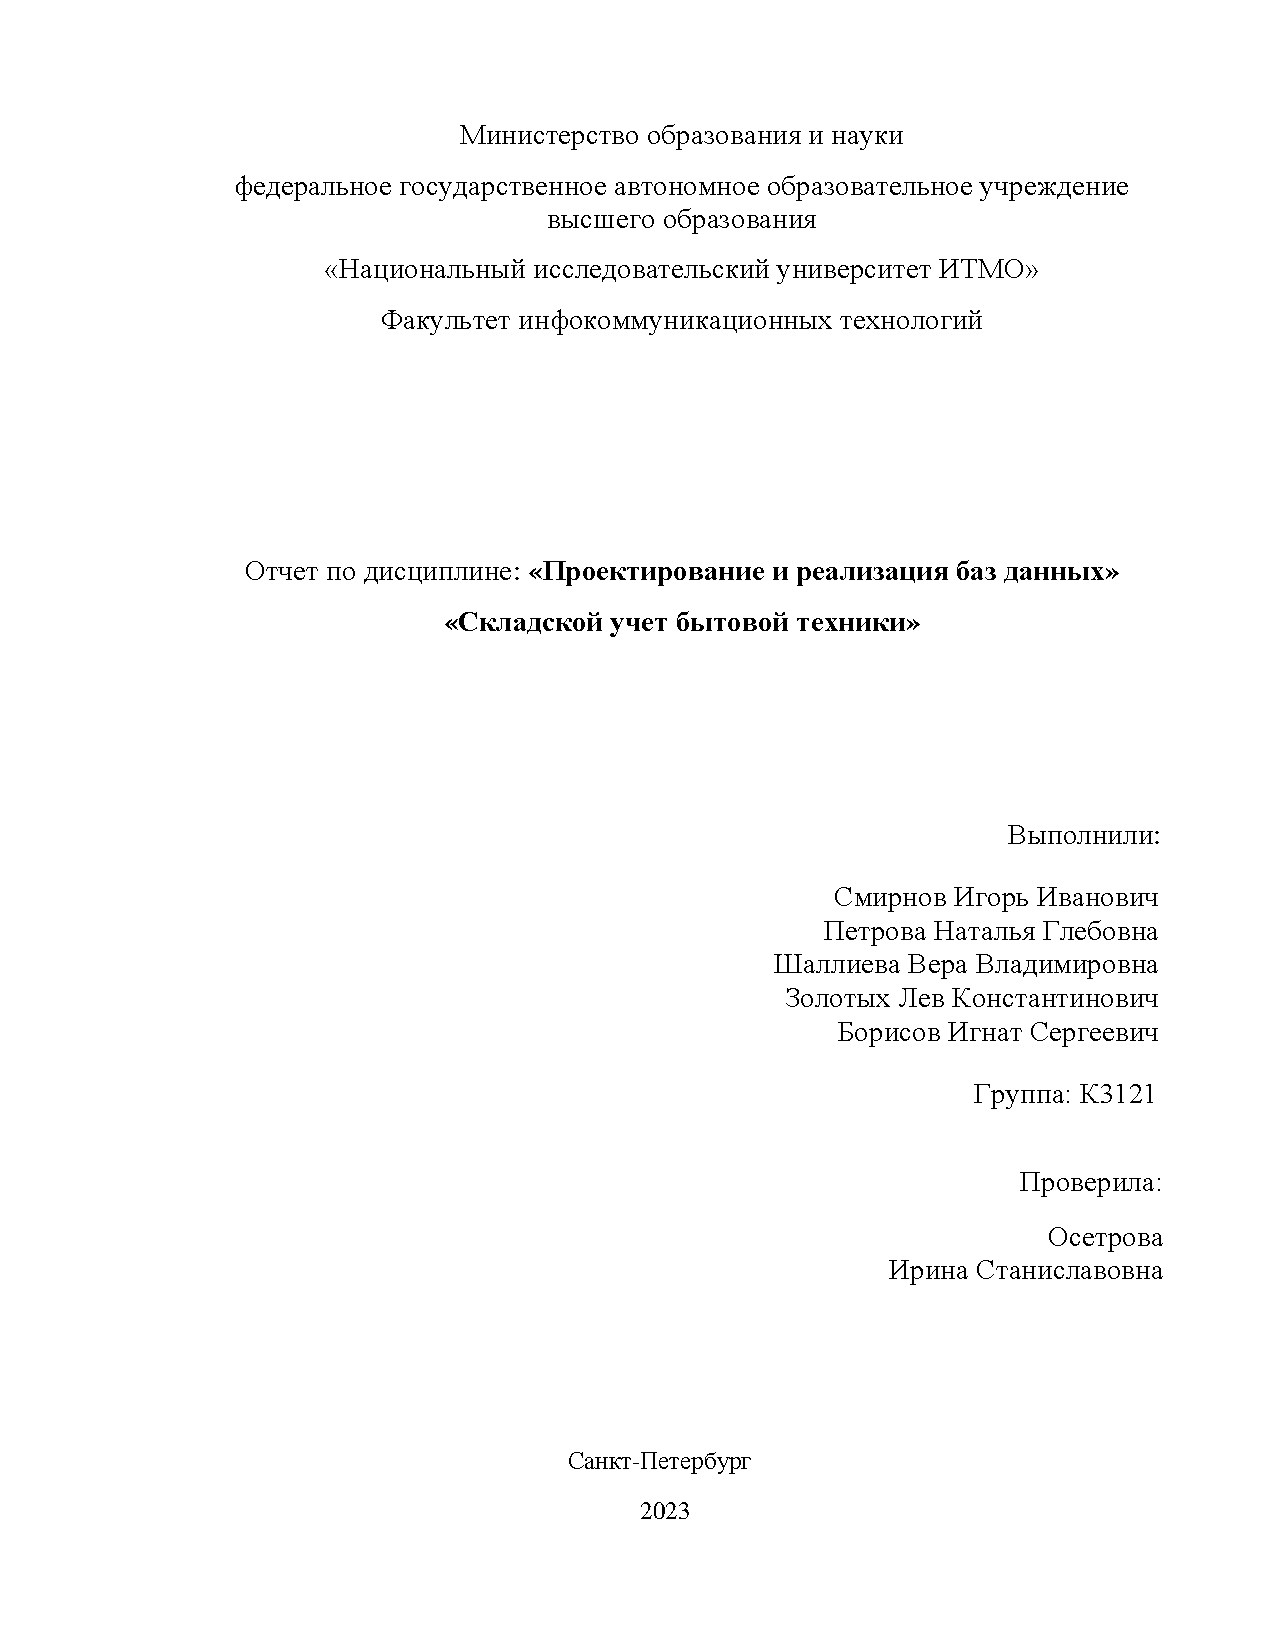
\includepdf[pages=-,pagecommand={}]{TitulBD.pdf}

\pagestyle{plain} % включаем нумерацию

\tableofcontents

\intro\label{intro}

Ведение складского учета бытовой техники - это необходимое условие для эффективного управления складскими запасами. Ведение учета позволяет получить точную информацию о количестве и типе техники на складе, а также контролировать ее движение и избежать потерь или краж.

Кроме того, ведение складского учета позволяет оптимизировать процесс продаж и сбыта, учитывая сезонность спроса на различные виды техники и особенности рынка. Например, знание того, какие товары на складе наиболее популярны в конкретный период, позволяет оперативно реагировать на изменения спроса и увеличивать прибыльность бизнеса.

Более того, точный учет бытовой техники на складе помогает улучшить качество обслуживания клиентов. Знание наличия техники на складе позволяет оперативно реагировать на запросы и желания клиентов, улучшать время доставки и решать проблемы с запасами.

В целом, ведение складского учета бытовой техники - это необходимый элемент эффективного управления складскими запасами, что позволяет улучшить качество обслуживания клиентов, увеличить прибыльность бизнеса и оптимизировать процесс продаж и сбыта.




Целью данной лабораторной работы является разработка логической схемы БД для бизнес-приложения «Складской учет бытовой техники».


Для достижения поставленной цели необходимо выполнить следующие задачи: 

1.	Исследовать предметную область. Формализовать предметную область. 

2.	Выявить основные сущности и их атрибуты. 

3.	Связать сущности (отношения). 

4.	Получить логическую схему.

\chapter{ВЫПОЛНЕНИЕ}
Объектом проекта является магазин бытовой техники, имеющий физические точки продажи. Когда речь идет о складской технике, учет на точечных магазинах является более актуальным, чем на онлайн-магазинах по нескольким причинам:

1. Физические склады: Точечные магазины имеют физические склады, где хранятся товары. В то время как в онлайн-магазинах товары хранятся на центральном складе и доставляются клиентам по мере необходимости. Поэтому учет складской техники на точечных магазинах является более актуальным.

2. Различные типы складской техники: Различные типы складской техники используются для различных целей, например, погрузочные машины используются для перемещения тяжелых грузов, а погрузчики с низким подъемом используются для перемещения грузов на низких высотах. На точечных магазинах обычно используется широкий спектр складской техники, поэтому учет их использования является более актуальным.

3. Контроль за состоянием техники: Точечные магазины обычно имеют своих сотрудников, которые могут следить за состоянием складской техники и проводить регулярное техническое обслуживание. В то время как в онлайн-магазинах такой контроль является более сложным, так как техника находится на центральном складе.

В целом, учет складской техники на точечных магазинах является более актуальным, так как они имеют физические склады и используют различные типы складской техники для различных целей.


В процессе разработки БД было выделено множество сущностей (рисунок 2).  Описание основных сущностей представлены в таблице 1.

1. Сущности (таблица построена по данным ERR-диаграммы (рисунок 2)):
\newpage
\begin{center}
\begin{longtable}{ |m{3cm}|m{5cm}|m{8cm}| } 
 \hline
 Сущность & Описание & Атрибуты \\ [0.5ex] 
 \hline\hline
 Товар & 
 Отдельная единица бытовой техники, которую необходимо отслеживать на складе.& \begin{center}
    \begin{tabular}{ m{4cm} | m{3.35cm} }
     Наименование & VARCHAR(255) \\  \hline
     Модель & VARCHAR(255) \\   \hline
     Серийный номер & VARCHAR(255) \\ \hline
     Модель & VARCHAR(255) \\   \hline
     Производитель & VARCHAR(255) \\   \hline
     Дата поставки & DATE \\   \hline
     Дата последней продажи & DATE \\   \hline
     Цена закупки & DECIMAL(10,2) \\  \hline
     Цена продажи & DECIMAL(10,2) \\ \hline
     Количество на складе & INT
    \end{tabular}
\end{center}\\
 \hline
 Поставщик & 
 Компания или организация, которая поставляет товар на склад. &
 \begin{center}
    \begin{tabular}{ m{4cm} | m{3.35cm} }
     Наименование & VARCHAR(255) \\  \hline
     Контактная информация & VARCHAR(255) \\   \hline
     Условия поставки & VARCHAR(255)
    \end{tabular}
\end{center}\\
 \hline
 Клиент & 
 Компания или физическое лицо, которое может приобрести товар на складе.&
  \begin{center}
    \begin{tabular}{ m{4cm} | m{3.35cm} }
     Наименование & VARCHAR(255) \\  \hline
     ФИО & VARCHAR(255)\\  \hline
     Контактная информация & VARCHAR(255) \\   \hline
     История покупок & VARCHAR(255)
    \end{tabular}
\end{center}\\
 \hline
 Поставка & 
 Операция, при которой товар поступает на склад от поставщика. &
 \begin{center}
    \begin{tabular}{ m{4cm} | m{3.35cm} }
     Дата & DATE \\  \hline
     ФИО & VARCHAR(255)\\  \hline
     Количество поставленного товара & INT \\   \hline
     Цена закупки & DECIMAL(10,2)
    \end{tabular}
\end{center} \\ 
 \hline
 Отгрузка & 
 Операция, при которой товар покидает склад. &
  \begin{center}
    \begin{tabular}{ m{4cm} | m{3.35cm} }
     Дата & DATE \\  \hline
     Количество покинувшего склад товара & INT\\  \hline
     Причина покидания товаром склада & VARCHAR(255)
    \end{tabular}
\end{center}\\
 \hline
 Продажа & 
 Операция, при которой товар продается клиенту. &
 \begin{center}
    \begin{tabular}{ m{4cm} | m{3.35cm} }
     Дата & DATE \\  \hline
     Количество проданного товара & INT\\  \hline
     Цена продажи & DECIMAL(10,2) \\   \hline
     Клиент & VARCHAR(255)
    \end{tabular}
\end{center}\\ 
 \hline
 Сотрудник склада & 
 Человек, который занимается учетом товаров на складе. &
 \begin{center}
    \begin{tabular}{ m{4cm} | m{3.35cm} }
     ФИО & VARCHAR(255) \\  \hline
     Контактная информация & VARCHAR(255)\\  \hline
     Должность & VARCHAR(255)
    \end{tabular}
\end{center}\\ 
 \hline
 Склад & 
 Место хранения товаров. &
  \begin{center}
    \begin{tabular}{ m{4cm} | m{3.35cm} }
     Наименование & DATE \\  \hline
     Адрес & VARCHAR(255)\\  \hline
     Площадь & DECIMAL(10,2) \\   \hline
     Вместимость & INT \\   \hline
     Сотрудники & VARCHAR(255)
    \end{tabular}
\end{center}\\ 
 \hline
 Категория товаров & 
 Группировка товаров по определенным критериям. &
  \begin{center}
    \begin{tabular}{ m{4cm} | m{3.35cm} }
     Наименование & VARCHAR(255) \\  \hline
     Описание & VARCHAR(255)
    \end{tabular}
\end{center} \\ 
 \hline
\end{longtable}
\end{center}


2. Связи:

Один к одному:
Каждая поставка связана с определенным поставщиком.

Каждая продажа связана с определенным клиентом.

Каждый сотрудник склада связан с определенным складом.

Один ко многим:
Каждый товар имеет поставщика.

Каждый товар относится к определенной категории товаров.

Каждый товар может быть продан клиенту.

Каждый склад имеет несколько категорий товаров.

Каждый склад может получать поставки от нескольких поставщиков.

Каждый клиент может совершать несколько покупок на складе.

Каждый сотрудник склада может быть ответственным за несколько категорий товаров.


Многие ко многим:
Каждый товар относится к определенному складу и имеет информацию о количестве на складе. (так как на одном складе может быть много товаров, и один товар может находиться на нескольких складах в разных количествах).


Таким образом была построена UML-диаграмма(рисунок 1), а также спроектирована модель базы данных для складского учета бытовой техники (рисунок 2).

\begin{center}
    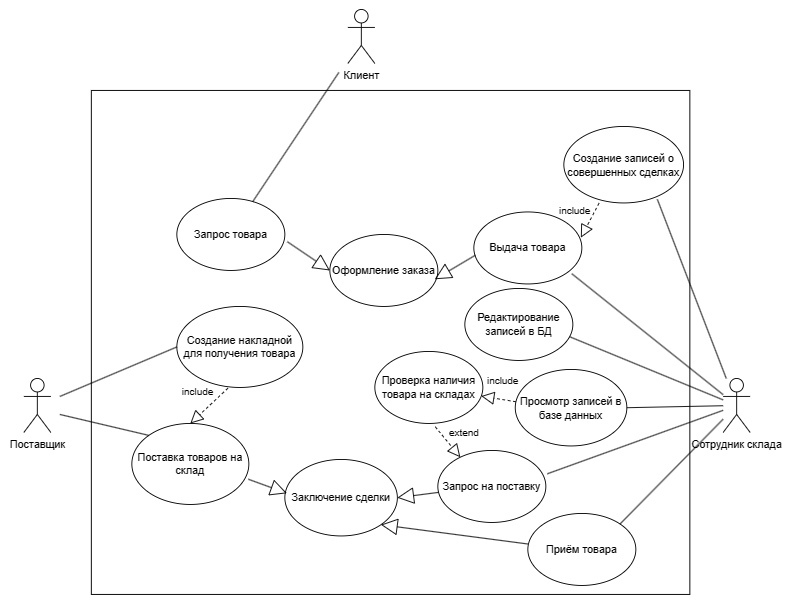
\includegraphics[scale=0.5]{UMLBD.jpg}

    Рисунок 1 - UML-Диаграмма
\end{center}

\begin{center}
    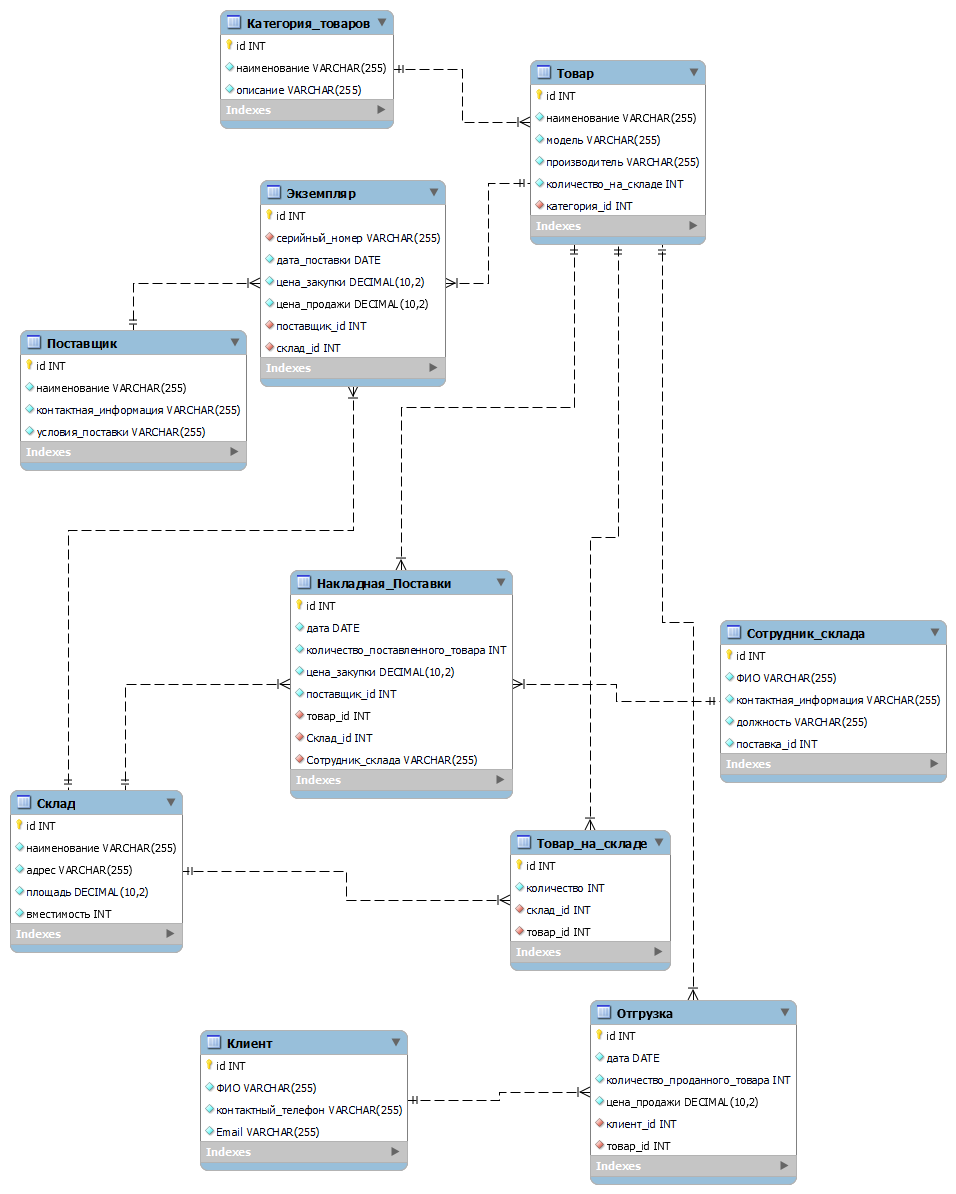
\includegraphics[scale=0.5]{Ispravlenniy_wid_dlya_bd_04_of_june.png}

    Рисунок 2 - Логическая схема БД
\end{center}



\conclusions

В ходе работы была исследована и формализована предметная область данного проекта. В процессе составления логической схемы были выявлены основные сущности — товар, поставщик, клиент, поставка, отгрузка, продажа, сотрудник склада, склад — и их атрибуты, описана связь между ними. Была использована одна UML-диаграмма (рисунок 1) и одна ERR-диаграмма (рисунок 2). Таким образом, результатом работы стала логическая схема БД для бизнес-приложения "Складской учёт бытовой техники". С развитием предприятия следует также развить и базу данных, например, добавить возможность определять транспорт для перевозки грузов и срочность заказов.


\begin{thebibliography}

\bibitem{bib1} Wikipedia: официальный сайт: 
\url{https://ru.wikipedia.org/wiki/База_данных} (Дата обращение 31.05.2023)

\bibitem{bib2} Wikipedia: официальный сайт: \url{https://ru.wikipedia.org/wiki/SQL} (Дата обращение 31.05.2023)

\bibitem{bib3} MySQL Workbench: официальный сайт: \url{https://dev.mysql.com/downloads/workbench/} (Дата обращение 31.05.2023)

\end{thebibliography}

\appendix
\chapter{}
\section{Смирнов Игорь Иванович}

\subsection{Эссе}

В современном мире базы данных распространены повсеместно. Без них
невозможно функционирование ни одной крупной информационной системы.Например, в любой социальной сети есть информация о собственном профиле пользователя, а также информация о профилях других людей. Вся эта информация хранится с помощью различных крупных баз данных. Однако с базами данных мы встречаемся каждый день не только в рамках взаимодействия с разлинчыми приложениями, такими как VK, YouTube и прочими.

Базами данных можно назвать и записные книжки не только в телефонах, но и в тетрадях у более старшего поколения. Ожидая автобус на остановке, мы также встречаемся с базой данных маршрутов, проходящих через эту остановку. Этот список можно продолжать до бесконечности, но все же есть еще один очень важный пример использования базы данных в повседневной жизни.
В образовании базам данных, конечно же, нашли применение. В первую
очередь это журнал класса, в котором стоят оценки учеников по разным
предметам. Для учеников в начале каждого учебного года выдают список предметов, который им предстоит изучить, а также на основе этого списка формируется расписание уроков и перемен. Подводя итог, в образовании базы данных применяют для структуривания информации об успеваемости учащиихся и нормировании учебного процесса.

Исходя из примеров выше, можно сделать вывод о пользе использова-
ния баз данных. Их важннейшей функцией является способность структу-
рировать всю имеющуюся информацию и представить ее в удобном для вос-
приятия виде. При этом такое представление может быть разным. Например, список класса всегда представлен в виде таблицы, а номера маршрутов могут быть представлены как в виде таблицы, так и в виде строки, в которой перечислены номера маршрутов. Имея такую структурированную информацию, реализация необходимых действий и достижение с их помощью поставленной задачи облегчается.
Несмотря на большую распространенность и полезность баз данных, у
них есть и свои минусы. Главный из них - риск потери информации. Причиной этому может служить ненадежный носитель или потеря носителя. Также в
случае слабой защищенности базы данных, информация из нее может попасть
в руки злоумышленников.

\subsection{Кейс}

Первым делом по утрам я, как и многие люди, проверяю уведомления на телефоне. Эти уведомления хранятся в небольшой базе данных, находящейся в памяти телефона. Точно так же можно описать и список контактов в телефонной книжке. Значит, множество небольших баз данных хранится у всех людей в их телефонах. В данном случае они помогают структурировать процесс получения новой информации и хранить старую в удобном для восприятия виде.

После пробуждения я мысленно пробегаю весь предстоящий день, вспоминая, где и когда у меня дела, оценивая их количество и свободное время между ними. Если свободного времени между делами достаточно, то я добавляю какое-то не срочное и необязательное на данный момент дело, которое можно успеть сделать во время получившегося перерыва. Обычно я это не записываю, но в целом если бы у меня была записная книжка, то она могла бы быть базой данных моих дел. В таком случае, база данных может оптимизировать процесс работы и повысить вероятность достижения поставленной задачи.

Почти каждый день я покупаю себе продукты и, чтобы грамотно рас-
порядиться деньгами и не забыть купить необходимые товары, составляю список того, что собираюсь приобрести. Такие записи формируют базу данных продуктов, которая помогает структурированно получить необходимую информацию, которая приведет к достижению поставленной задачи.

На практиках и лекциях я веду многостраничные конспекты. Это со-
ставляет базу данных полученной на занятиях информации, которая поможет мне во время подготовки к экзаменам. Такая база данных хранит информа-
цию до момента ее востребованности.

Периодически я ищу различные варианты проведения досуга в различ-
ных районах города. Найдя что-то интересное, я записываю информацию о

месте, цене и дате (разовое или ограниченное по времени мероприятие) в спе-
циальный файл. Такая база данных также помогает сохранить информацию до момента ее востребованности у пользователя.

Под конец дня, приготавливаясь ко сну, я готовлю будильник на утро. В
приложении уже есть импользованные мною заготовки для будильников, так
что такую систему можно назвать базой данных моих личных будильников.
Она содержит в себе информацию, которая влияет на состояние и работу
исполнителя.

\section{Шаллиева Вера Владимировна}

\subsection{Эссе}

В нашей современной жизни уже давно не в новинку такая вещь как базы данных. Но стоит всё же рассмотреть конкретную формулировку. База
данных — это совокупность структурированных данных, которые хранятся в
компьютерной системе и могут быть использованы для выполнения различных операций, таких как поиск, добавление, изменение и удаление данных.
Базы данных используются в различных областях, включая бизнес, науку,
медицину и другие сферы деятельности. Они позволяют эффективно хранить
и управлять большим объемом информации, а также обеспечивают быстрый
доступ к нужным данным.

Что же могут дать нам базы данных? Благодаря базам данных есть возможность хранить большие объемы информации и организовывать ее в соответствии с определенными правилами и структурами. Анализируя данные БД, быстрее принимаются те или иные решения из-за чёткости рассмотрения
и автоматизации процессов. Базы данных могут интегрироваться с другими
системами, такими как CRM, ERP и другие, что позволяет улучшить эффективность работы. А также они обеспечивают быстрый доступ к нужной
информации благодаря эффективной организации, индексированию данных
и обработки данных с помощью различных операций, таких как поиск, фильтрация, сортировка, агрегация и другие.

Сфера применения БД настолько огромна, что нельзя в полной мере описать всё. Но есть основные направления:

1. Банковские системы: Банки используют базы данных для хранения
информации о клиентах, их счетах, транзакциях и других финансовых операциях.

2. Торговые системы: Розничные магазины и интернет-магазины используют базы данных для хранения информации о продуктах, ценах, заказах и
доставке.

3. Социальные сети: Социальные сети используют базы данных для хранения информации о пользователях, их профилях, контактах и сообщениях.

4. Транспортные системы: Компании по перевозке грузов и пассажиров
используют базы данных для хранения информации о рейсах, маршрутах,
расписаниях и билетах.

5. Государственные системы: Государственные учреждения используют
базы данных для хранения информации о налогах, паспортах, правах на вождение и других документах.

6. Образовательные системы: Школы, колледжи и университеты используют базы данных для хранения информации о студентах, учебных планах,
оценках и преподавателях.

Но несмотря на все плюсы БД и обширность их применения естественно есть и минусы. А точнее риски, которые поджидают пользователей. Во-первых, недостаточная защита от вредоносных ПО и вероятность потери
данных. Если база данных не защищена должным образом, то данные могут быть утеряны из-за сбоев в системе, а так же есть риск утечки данных
злоумышленникам. Во-вторых, неправильная обработка данных и проблемы
совместимости. Некорректная обработка данных может привести к ошибкам
и неправильным выводам. И если база данных несовместима с другими системами, то это может привести к проблемам при интеграции.

В целом, базы данных играют важную роль в повседневной жизни людей
и бизнеса. Они помогают сохранять и обрабатывать большие объемы информации, упрощать процессы и повышать эффективность работы. Они очень
важны в современной жизни.

\subsection{Кейс}

Каждый мой день весьма насыщен разными поездками, событиями и действиями. И если не задумываться, то можно и не заметить, как везде проскакивает использование баз данных. Они повсюду.

Начиная свой день с проверки телефона, что очень плохо, но как факт
отрицать нельзя. Мне хочется посмотреть ИСУ Университета ИТМО, тут и
есть уже применение, просмотр баз данных. В образовании БД используются
для хранения информации о студентах, учебных планах и другой важной информации. После я вспоминаю о том, что грядёт много праздников и нужно
покупать подарки. Захожу в сервис "OZON"для заполнения корзины покупками. Это одна сплошная база данных, где можно просмотреть все параметры
каждой позиции, почитать множество отзывов, изучить продавцов, а также
внесённые данных карты тоже попадут во взаимодействие с БД.

Выходя из общежития, я использую пропуск и меня вносят в базу данных "вышедших аналогично по моему возвращению. Такой же принцип работы мы наблюдаем на турникетах университета при входе/выходе. И вот я
уже в университете, между парами я хочу написать эссе по дисциплине "Базы данных но для начала нужно изучить предметную область. Я пользуюсь
поисковиком и это тоже огромная база данных, где можно найти любую информацию. Но любая работа идёт лучшее под музыку и воспользовавшись
музыкальным сервисом, передо мной стоит задача просмотреть музыкальную
БД и найти любимый трек.

Пары окончены и моему организму требуется пополнить силы и сходить
перекусить. Зайдя в популярную кафешку, я вижу табло для самостоятельного заказа, где из базы данных, а то есть из меню, я выберу свой заказ. И
после плотного обеда, мне предстоит собраться с друзьями у меня дома и посмотреть фильм. Мы выбрали сервис -онлайн кинотеатр "Кинопоиск HD где
естественно тоже применены базы данных, просматривали множество категорий, сортировали по любимым жанрам и т.д.

Время было проведено хорошо, но и о важных вещах не стоит забывать,
а то есть о своём здоровье. У меня был намечен поход ко врачу. Придя в поликлинику, я в табло выдала себе талончик. Для проверки занятости врачей,
сопоставления расписания работы, распределение кабинетов использовалась
внутренняя БД. Непосредственно у врача заполнялась моя медицинская карта, в наше время это делается на компьютере. И это демонстрирует использование БД для хранения медицинских записей, результатов анализов и другой
информации о пациентах.

Из вышеперечисленных примеров можно однозначно доказать все высказывания о безграничности использования баз данных, об их необходимости
применения в нашей нелёгкой жизни каждый день.

\section{Петрова Наталья Глебовна}

\subsection{Эссе}

С появлением первых компьютеров базы данных стали неотъемлемой частью вычислительной техники. Невозможно представить ни одной сферы жизни без использования баз данных, которые помогают значительно упростить и автоматизировать все внутри происходящие процессы. Самое удивительное, что мы ежедневно встречаемся с БД, даже не подозревая об этом. Но прежде, чем конкретизировать сферы использования, нужно разобраться, что вообще из себя представляют БД?

Существует множество разных вариаций и определений понятия «базы данных», но если обобщить, то базы данных — это набор структурированных данных, а структурированы они по каким-то определенным параметрам, которые объединяют их. Как правило БД записывают как таблицу, состоящую из строк и столбцов. Но при этом базу данных нельзя назвать полноценной программой, это больше похоже на файл, в котором хранится информация, но, чтобы получить эти данные необходима программа, которая будет управлять этой базой данных (СУБД). Таким образом, можно сделать вывод о том, что БД — это файлик, который хранится на диске компьютера, а СУБД — это инструменты, посредством которых осуществляется управление этими базами.

Область применения баз данных на сегодняшний день необъятна, они используются везде, начиная с банковской сферы и заканчивая производственной. Они создаются во всех предприятиях малого, среднего и крупного бизнеса: в банках, пенсионных, страховых, благотворительных и иных фондах. Масштабы применения БД могут быть очень обширными - от небольших для настольных компьютеров до крупных хранилищ, доступ к которым не так легко получить.

Широко базы данных используются в сфере образования для хранения информации о студентах, учителях, учебных планах и расписаниях занятий. Базы данных могут также содержать информацию об успеваемости студентов, оценках, присутствии и результаты экзаменов. Благодаря базам данных учителя могут быстро находить информацию о студентах, их успеваемости и посещаемости, а также следить за их учебным прогрессом. Базы данных также используются для разработки учебных материалов и учебных планов. Учебные материалы могут включать тексты, видео и аудио материалы, изображения и многие другие типы данных. Благодаря базам данных учителя могут быстро находить необходимый учебный материал и использовать его в своей работе.

Использование БД имеет как свои преимущества, так и недостатки. Если говорить о плюсах, то в первую очередь это удобство и быстрота получения необходимой информации, во-вторых, поддерживается целостность данных и уменьшается безопасность их утечки. Помимо этого, немаловажным является контроль за избыточностью и повышение эффективности с ростом масштабов системы, что достигается за счет использования СУБД.

Хотя базы данных имеют множество преимуществ и широко используются во многих сферах, они также имеют свои недостатки и ограничения. Первым недостатком является сложность создания и обслуживания баз данных. Создание базы данных требуют значительного объема времени и ресурсов, необходимо постоянно обновлять их содержимое и защищать от потенциальных угроз безопасности. Еще одним недостатком баз данных является их ограниченность. Базы данных ограничены в том смысле, что они могут хранить только определенный тип данных и ограниченный объем информации.

В заключении хотелось бы отметить, что базы данных являются неотъемлемой частью нашей жизни и играют важную роль в различных сферах. Они помогают улучшать качество обслуживания клиентов, повышать эффективность производственных процессов, улучшать результаты медицинских исследований, а также улучшать процессы управления в государственных органах.

\subsection{Кейс}

В наше время мы часто используем базы данных, даже не задумываясь об этом. Как и многие другие люди, я использую базы данных в повседневной жизни для облегчения своих задач и получения необходимой информации.

Приведу несколько примеров, где мы ежедневно сталкиваемся с использованием БД. Одним из примеров, является использование баз данных при работе с почтой. Когда я отправляю письмо или пользуюсь электронной почтой, все мои сообщения сохраняются в базе данных, чтобы я могла легко находить старые сообщения и восстанавливать данные в случае необходимости. Кроме того, я использую базы данных для поиска информации. Например, если я ищу рецепт определенного блюда или ищу информацию о новостях, то я могу воспользоваться поисковой системой, которая обращается к базам данных, чтобы найти необходимую информацию. Это позволяет мне быстро и легко находить ответы на свои вопросы и решать различные задачи. Базы данных также играют важную роль при использовании социальных сетей. Когда я пользуюсь социальными сетями, все мои сообщения, комментарии и фотографии сохраняются в базах данных, которые позволяют мне легко находить старые сообщения и управлять своими настройками безопасности. 

Наконец, я использую базы данных для управления своими личными данными. Я храню свои личные данные, такие как паспортные данные, налоговые документы и контактные данные, в базе данных, которую я легко могу обновлять и использовать для различных целей. 

В целом, базы данных играют важную роль в повседневной жизни, даже если мы не осознаем это. Они облегчают нашу жизнь, позволяя нам быстро находить и управлять информацией, которая имеет для нас значение. Благодаря использованию баз данных мы можем значительно экономить свое время и увеличивать свою эффективность в повседневных задачах. Они позволяют ускорить и упростить многие процессы, связанные с хранением и поиском информации, что делает их важным инструментом в нашей повседневной жизни.

\section{Борисов Игнат Сергеевич}

\subsection{Эссе}

Человек начал использовать своеобразные базы данных задолго до появления компьютеров. Неудивительно — имелся огромный, непомерный массив информации, который нужно было хранить, обрабатывать и отвечать на запросы пользователей, клиентов и любых других людей, а то и компаний, которые имели на это право. Несмотря на отсутствие компьютеров, люди всё равно обрабатывали всю эту информацию, храня её на бумаге, что, конечно, значительно хуже и медленнее компьютерной базы данных, но это всяко лучше, чем не хранить информацию никак. Но что же всё-таки эта «база данных»?

В современном мире базы данных, как и любое другое понятие, имеют множество всевозможных определений, но все эти понятия можно консолидировать в следующее определение: «набор структурированных по определённым параметрам данных, объединяющих эти данные». Базу данных зачастую хранят в виде таблиц. Базу данных нельзя назвать программой, так как это по сути файл, хранящий в себе информацию, но не выдающий её сам по себе — для извлечения данных нужна отдельная программа, которая и будет управлять данной базой данных — система управления базой данных, сокращённо СУБД. Таким образом, база данных — не программа сама по себе, а только файл, вместилище информации, которую можно достать с помощью СУБД.

Базы данных используются сегодня практически во всех сферах деятельности человека, начиная с заводов и заканчивая школами. На заводе база данных хранит всю информацию о станках, их деталях, производственных мощностях, продукции и самих рабочих, в школах база данных хранит список учащихся, их параметры и данные, оценки, хранит данные учителей и параметры программы образования. Благодаря базам данных владельцы предприятия могут понять, какую часть производства им нужно развивать, а родители могут легко проверить успеваемость своего ребёнка — ученика вышеупомянутой школы, и быстро принять необходимые меры, если ребёнок начнёт хуже понимать тот или иной предмет. В университете студент может быстро и без лишних трудностей узнать свою успеваемость, стипендию, расписание предметов и прочее — всё это с помощью баз данных.

Однако у всего есть как положительная, так и отрицательная сторона, и базы данных здесь не исключение. Преимущества очевидны и велики — невероятно ускоряется и облегчается практически любой труд, обеспечивается безопасность данных.

Но есть и серьёзные недостатки: базы данных не всесильны и не появляются из ниоткуда, их сначала нужно создать, и чем более база данных сложна и объёмна, тем дольше и труднее её создавать. Также к базе данных при неудачном стечении обстоятельств может получить доступ злоумышленник, и он получит данные сразу к целому массиву информации, ввиду чего защита баз данных должна постоянно совершенствоваться, что требует сил, времени и средств.

Суммируя всё сказанное, стоит заметить, что на базах данных построен практически весь обмен информацией в современном мире, ввиду чего они крайне важны в жизни человека. Именно базы данных упрощают быт многократно, помогаю человеку экономить своё время и тратить его на всевозможные полезные дела.

\subsection{Кейс}

В современном мире базы данных используются крайне активно и повсеместно. Хотя не знающему человеку может показаться, что он с ними никак не связан, на самом деле базы данных буквально пронизывают всю нашу жизнь.

Приведу несколько примеров, иллюстрирующих повсеместность баз данных. Один из примеров — не что иное, как самый обыкновенный и привычный интернет-магазин. Когда я захожу на сайт того или иного интернет-магазина с целью купить что-то или даже просто посмотреть ассортимент, я на самом деле обращаюсь к удалённой базе данных, хранящей информацию обо всех товарах данного магазина, обо всех учётных записях пользователей, обо всех партнёрах магазина и прочую всевозможную информацию. Также я использую базы данных для поиска того или иного учебного материала — когда я набираю текст в поисковой системе, на самом деле я отправляю запрос базе данных на выдачу мне наиболее подходящих результатов, которые отправляются мне на компьютер и отображаются на экране.

Наконец, я использую базы данных для того, чтобы получать всевозможные документы, оформлять официальные запросы, уточнять информацию на сайте Госуслуг, который также содержит в себе базы данных, содержащих всю вышеуказанную информацию, запросы к которой я на самом деле и оформляю.

Как видите, базы данных играют действительно немыслимую роль в жизни человека, даже если он не признаёт этого. Базы данных позволяют выполнять практически безграничное количество задач, позволяют получить доступ к фактически любой информации в считанные секунды, минуя необходимость искать ту или иную информацию вручную, лично. Именно базы данных позволяют автоматизировать колоссальное количество задач, как монотонных, так и в значительной мере интеллектуальных. Без баз данных наша жизнь была бы совсем другой, гораздо тяжелее того, что мы имеем с ними. Все эти свойства баз данных делают их одним из важнейших инструментов в нашей жизни.

\section{Золотых Лев Константинович}

\subsection{Эссе}

Сегодня базы данных встречаются нам повсюду, и обусловлено это тем, что это самый удобный способ не только хранения большого количества информации, но и работы с ней.

Говоря “повсюду”, я ничуть не преувеличивал. Любая социальная сеть хранит данные своих пользователей в виде баз, большинство магазинов (как работающих онлайн, так и имеющих торговые точки), используют базы данных для учёта товаров, базы данных обширно используются банками. Интересное применение базам данных было найдено в шахматном спорте: в открытом доступе лежат десятки тысяч партий, позволяя каждому учиться на них, либо найти партии своего соперника по партии и подготовиться к поединку.

Использование баз данных не обошло стороной и сферы образования. Поскольку всё чаще дневники переходят в электронный вид, появляется необходимость хранить информацию о множестве учеников: их оценки, расписание, контакты для быстрой связи. Студентам нужно то же самое, но в расширенном виде. Например, в университете ИТМО студент может выбрать для себя разные спортивные секции, места в которых ограничены, а это значит, что помимо базы данных хранения профиля самого студента, нужна база для хранения информации о каждой секции. То же самое касается переговорных помещений в комнатах для совместной работы. В базе данных профиля студента может храниться информация о его читательском билете, но должна быть и база самой библиотеки, в которой будет указано, например, какие книги в наличии есть, а каких нет, и когда появятся последние. И это лишь малая часть возможного применения баз данных в сфере образования.

Ценность возможностей, которые приобретает пользователь базы данных сложно переоценить. В основном эти возможности заключаются в экономии времени. Можно быстро узнать какую-либо интересующую пользователя информацию, если она хранится в открытом доступе. Также базы данных позволяют выполнить некоторые действия, также экономя время (например, покупки).

К сожалению, помимо бесспорного удобства базы данных могут нести в себе и некоторую опасность. Это может являться следствием её неудачного проектирования или её повреждения. Первое может привести к тому, что в базе данных, к которой есть открытый доступ лежит какая-либо конфиденциальная информация её пользователей. Некоторые базы данных должны быть полностью скрыты от посторонних глаз. Ярким примером является банк. Если кто-либо извне узнает любую информацию пользователя, кроме его имени, то это может привести к краже денежных средств со счёта последнего. Неактуальность или потеря данных также являются важными проблемами, с которыми пользователи могут столкнуться. Например, интернет магазин должен быстро обновлять информацию о количестве товара. Если он в избытке, то проблем может и не быть, но если товара почти не осталось, то важно, чтобы заказов было не больше, чем его количество. Потеря данных может же произойти по разным причинам, поэтому важно, чтобы базы были от этого защищены (возможно, копированием), а сам пользователь самую важную информацию лично дублировал у себя, ведь записные книжки себя ещё не исчерпали.

В качестве заключения хочу сказать, что базы данных в разы упрощают жизнь. Вместо поиска шахматной партии по сотням книг и архивов, можно просто вбить фамилии игроков и получить доступ к ней, почти любой товар можно купить в один клик, не выходя из дома, а читательский билет теперь невозможно потерять или забыть. Однако, окончательно от старых методов хранения информации отказываться пока не стоит, ведь от потери данных на данный момент целиком никто не застрахован.

\subsection{Кейс}

Можно сказать, что я начинаю использовать базы данных, как только я беру в руки телефон. Если я хочу кому-то позвонить из списка контактов, то этот самый список является, пусть маленькой и несложной, но базой данных. Если я использую какое-либо приложение, то у меня в нём есть аккаунт, информация о котором хранится в соответствующей базе, будь то социальная сеть, игра, кино и так далее.

Если в течение дня у меня появляется свободное время, то я играю на барабанах. Для этого мне нужно либо приложение для прослушивания музыки, чтобы играть любимые песни, либо специальные приложения, в которых содержатся табулатуры, необходимые для того, чтобы я мог выучить сложные партии, которые на слух запомнить и разобрать не получается. В обоих приложениях композиции хранятся в базах данных. В первом случае они могут храниться в качестве элементов плейлистов, альбомов или треков конкретного исполнителя, во втором же у них нет особых разделений, но сами композиции помимо названия, времени, исполнителя, содержат нотные записи.

Поскольку я студент, то каждый день пользуюсь ИСУ, который очень сильно облегчает мне жизнь. В нём можно посмотреть расписание занятий, забронировать переговорную комнату, записаться на секцию, узнать свою успеваемость, предстоящие события и многое другое. Всё вышеперечисленное хранится в разных базах данных, позволяя мне быстрее, проще и более качественно распределять время.

Поскольку я более четырнадцати лет играю в шахматы, то у меня есть опыт работы и с шахматными базами данных. На самом деле в этом нет ничего сложного: Достаточно вбить фамилии и инициалы игроков в специальное приложение ”ChessBase”, и оно выдаст партии, подходящие под условия поиска, которые были в неё занесены. В своё время это был настоящий прорыв в шахматном спорте, потому что теперь стало гораздо проще подготовиться к партии с соперником, просматривая его игры, стало проще изучать шахматные аспекты по партиям великих, ведь все они хранятся в открытом доступе, а сама база может регулярно пополняться любым пользователем, имеющим соответствующую лицензию: достаточно просто вбить ходы партии и, если необходимо, информацию об играющих (не только инициалы,но и их рейтинг) или самой партии (дата, название турнира, номер тура, результат).

Если я иду есть, то для оплаты я использую банковскую карту, информация о которой хранится в базе данных. Также возможно, что для быстрого заказа или участия в бонусной программе я буду использовать приложение, тогда мой профиль, список покупок и моё количество баллов тоже будут храниться в базах данных.

Из вышесказанного можно сделать вывод, что каждый день мы используем базы данных, возможно даже, сами того не замечая. В моём случае оказались охвачены самые разные сферы жизни, в которых эти базы данных используются: образование, досуг, спорт, сфера услуг. Везде базы данных сильно упрощают нам жизнь, особенно, если научиться ими пользоваться.

\chapter{}

\section{Распределение обязанностей участников}

\subsection{Смирнов Игорь Иванович}

Анализ выделенного кейса и написание по нему эссе.

Распределение заданий между всеми участниками, внесение правок в отчет, курирование построение логической схемы базы данных.

\subsection{Шаллиева Вера Владимировна}

Анализ выделенного кейса и написание по нему эссе.

Определние сущностей и связей, построение логической схемы базы данных, внесение правок в отчет.

\subsection{Петрова Наталья Глебовна}

Анализ выделенного кейса и написание по нему эссе.

Определние сущностей и связей, построение UML-модели, внесение правок в отчет.

\subsection{Борисов Игнат Сергеевич}

Анализ выделенного кейса и написание по нему эссе.

Поиск информации, техническое обеспечение, внесение правок в отчет.

\subsection{Золотых Лев Константинович}

Анализ выделенного кейса и написание по нему эссе.

Написание отчета, участие в проектировании UML-модели.






\end{document}
